\chapter{PSkel-MPPA}
\label{cha:proposta}

Esta seção apresenta as ideias fundamentais que irão embasar a proposta e implementação
da adaptação do \fw \pskel para o processador \mppa.

\section{Visão Geral}

Como dito anteriormente, diversas dificuldades prejudicam o desenvolvimento de aplicações para
processadores \textit{manycore}, tais como o \mppa. Neste projeto, será dado um enfoque para
uma classe de aplicações paralelas que seguem o padrão \stencil. Nesse sentido, adaptar
o \fw PSkel para esse processador trará benefícios claros, simplificando o desenvolvimento
de aplicações \stencil para o \mppa. O \fw fornecerá uma transparência
no particionamento de tarefas e dados para esse ambiente, liberando o desenvolvedor
da utilização de meios de comunicação via \noc. Além disso, aplicações já desenvolvidas para o
\fw poderão ser executadas no \mppa sem a necessidade de nenhuma alteração em seus códigos originais.

% \todo[inline]{Destacar o que consiste a proposta: 1) que classes serão alteradas? 2) como será feita a comunicação dos dados? 3) será feito uso de técnicas para divisão dos tiles? quais? 4) será dado foco somente para desempenho? ou consumo de energia também? Os resultados obtidos serão comparados com quais outras arquiteturas?}

A nova adaptação do \fw suporta matrizes \stencil 2D, adotando o modelo
mestre-trabalhador. O processo mestre é executado no subsistema de \es conectado
à uma memória LPDDR3, alocando dados de entrada e saída. Por outro lado, o
processo trabalhador é executado em cada \textit{cluster} com o
objetivo de realizar a computação \stencil de forma paralela. Devido às
limitações de memória no \mppa, o mestre deverá enviar para o trabalhador
pequenas partições da matriz de entrada, denominadas de \textit{tiles}. Durante
o processo de subdivisão, cada \textit{tile} deverá considerar as dependências
de vizinhança intrínsecas do padrão \stencil. Mais precisamente, a computação
realizada sobre um elemento de um certo \textit{tile} poderá possuir uma relação
de dependência com outros \textit{tiles} devido à máscara da computação.

Para tratar os problemas de dependência foi utilizada a técnica de
\textit{tiling} trapezoidal~\cite{meng11} na solução proposta, resultando em redundância de
dados e computações~\cite{Rocha:2017}. Mais especificamente, \textit{tiling} é
geralmente utilizado para particionar a computação de uma aplicação \stencil em
partes menores (\textit{tiles}) entre \textit{clusters}. Essa subdivisão
tem como objetivo possibilitar a execução paralela da aplicação.

Contudo, o processo de \textit{tiling} introduz problemas de dependência, pois,
para computar os elementos das bordas de um \textit{tile}, é necessário obter
os valores resultantes em outros \textit{clusters}. A Figura~\ref{fig:tilingHalo} ilustra
esse comportamento. As regiões que precisam ser resolvidas por sincronizações e
comunicações entre \textit{clusters} é denominada região \textit{halo}. Dependendo do número
de sincronizações e comunicações realizadas, a aplicação pode demorar um tempo
considerável realizando o particionamento de dados entre \textit{clusters}, prejudicando o
desempenho da aplicação.

\begin{figure}[!h]
	\centering
    \caption{Esquemático ilustrando a região \textit{halo}.}
    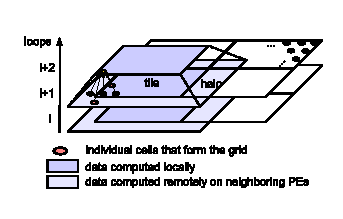
\includegraphics[width=0.6\textwidth]{figs/tilingHalo.pdf}
    Fonte:~\cite{meng11}.
    \label{fig:tilingHalo}
\end{figure}



Para contornar essa sobrecarga após cada iteração, um \textit{tile} pode ser
alargado para incluir uma \textit{ghost zone}. A Figura~\ref{fig:tiling} ilustra
essa alternativa, onde a \textit{ghost zone} alarga o \textit{tile}, fazendo-o
sobrepor \textit{tiles} vizinhos por meio de múltiplas regiões \textit{halo}.
Desta forma, \textit{clusters} podem gerar mais sobreposições com quantidade proporcional ao
número de iterações da aplicação. Além disso, a mesma figura ilustra o
comportamento da \textit{ghost zone}, onde ela agrupa as iterações em estágios.
Cada estágio realiza operações sobre \textit{tiles} sobrepostos, denominados
trapezóides. Por fim, os trapezóides irão produzir um dado sem sobreposição ao
final da computação de todas as iterações.

\begin{figure}[!h]
	\centering
    \caption{Esquemático ilustrando a \textit{ghost zone}.}
    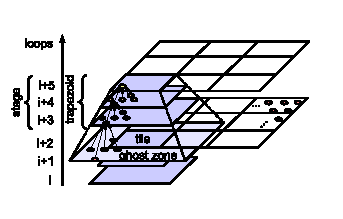
\includegraphics[width=0.6\textwidth]{figs/tiling.pdf}
    Fonte:~\cite{meng11}.
    \label{fig:tiling}
\end{figure}



A seguir, a técnica será ilustrada mais profundamente
por meio de definições formais. Seja $A$ uma matriz de dados 2D, com dimensões
$\textrm{dim}(A) = (h,w)$, onde $w$ e $h$ são largura e altura, respectivamente.
Utilizando \textit{tiles} de dimensões ($w'$, $h'$), é possível obter
$\lceil\frac{w}{w^\prime}\rceil\lceil\frac{h}{h^\prime}\rceil$ \textit{tiles}
sobre $A$. Seja $A_{i,j}$ um \textit{tile} seguindo as definições descritas,
onde $0 \leq i < \lceil\frac{w}{w^\prime}\rceil$ e $0\leq j <
\lceil\frac{h}{h^\prime}\rceil$. $A_{i,j}$ possui um \textit{offset} $(i
w^\prime, j h^\prime)$ relativo ao canto superior esquerdo de $A$ e
$\textrm{dim}(A_{i,j}) = (\min\{w^\prime, w-i w^\prime\}, \min\{h^\prime, h-j
h^\prime\})$. O \textit{offset} é um índice de deslocamento necessário para
acessar os elementos de um \textit{tile}.

A Figura~\ref{fig:block2d} ilustra a técnica de \textit{tiling} trapezoidal. Um
\textit{tile} lógico (linha sólida interna) é contido em uma matriz de dados 2D
(linha pontilhada externa) com \textit{offsets} verticais e horizontais dados
por $jh^\prime$ e $iw^\prime$. Se $t$ iterações de uma aplicação \stencil
precisam ser realizadas, é possível computar $t^\prime$ iterações consecutivas
sobre $A_{i,j}$ ($t^\prime \in \left[1,t\right]$) sem a necessidade de nenhuma
troca de dados entre \textit{tiles} adjacentes, isto é, $t^\prime$ iterações
internas. Para realizar iterações consecutivas é necessário utilizar um
\textit{tile} lógico ($A_{i,j}$) alargado com uma \textit{ghost zone} (área
entre a linha sólida interna e a linha sólida externa) que possui uma
\textit{halo region} (área entre a linha sólida interna e a linha pontilhada
interna). Seja $r$ o maior deslocamento necessário sobre a vizinhança de um
elemento, determinado pela máscara \stencil. A área com alcance $r$ que contém a
vizinhança é denominada \textit{halo region}. O número de \textit{halo regions}
que compõem a \textit{ghost zone} é proporcional à $t^\prime$. Desta forma, o
\textit{tile} alargado $A^\ast_{i,j}$ possui um \textit{offset} $(\max\{iw^\prime -
rt^\prime, 0\}, \max\{jh^\prime - rt^\prime, 0\})$ relativo à $A$. Portanto,
existe um \textit{trade-off} entre o custo de computação redundante e o número
de comunicações e sincronizações na \noc durante o processamento de computações
\stencil iterativas no \mppa.

\begin{figure}[!h]
  \begin{minipage}[b]{0.9\textwidth}
	\centering
	\caption{2D tiling~\cite{Rocha:2017}.}
    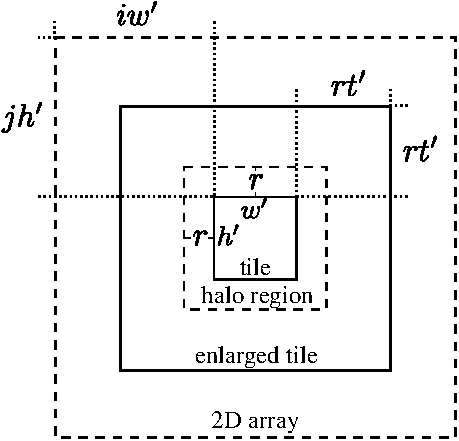
\includegraphics[height=5cm]{figs/tile.pdf}
	\label{fig:block2d}
  \end{minipage}
\end{figure}



% Na implementação da proposta será necessário modificar classes já existentes
% no \fw para suportar as características do \mppa. Devido à subdivisão da matriz de entrada
% e a comunicação serem diferentes para o \mppa em relação à comunicação
% \cpu-\gpu, classes responsáveis por essas
% operações devem ser modificadas, como, por exemplo, a classe que determina a estrutura
% \textit{Stencil}. Além disso, a comunicação entre os processos mestre e escravo
% do \mppa será feita utilizando portais de comunicação.

% Mais especificamente, uma nova função responsável por subdividir a matriz
% de entrada em pequenas partes (\textit{tiles}), será criada.
% Os \textit{tiles} serão construídos seguindo uma técnica de \textit{tiling}
% trapezoidal~\cite{meng11}, sendo enviados para o processo trabalhador seguindo um modelo de
% escalonamento de tarefas do tipo \textit{round-robin}.
% Para efetuar o envio dos \textit{tiles} será criado um portal de comunicação relacionado com
% cada \textit{tile} da matriz de entrada.
%
% A técnica trapezoidal permite o mestre enviar \textit{tiles} aumentados, isto é,
% \textit{tiles} com uma borda maior, determinada por uma \textit{ghost zone}.
% Desta forma, o processo trabalhador poderá realizar mais de uma iteração sobre
% cada \textit{tile}, diminuindo o número de sincronizações entre os processos.

% A Figura~\ref{fig:tiling} ilustra as modificações sobre o \textit{tile} alargado
% em relação às iterações consecutivas. Mais es

% Devido ao \textit{tile} ser acrescido de uma parte da matriz atribuída a outro
% \textit{tile}, computações redundantes serão realizadas. O tamanho do
% \textit{tile} aumentado pode trazer perda em desempenho em troca de um menor
% número de comunicações entre os processos, isto é, quanto maior o número de
% computações redundantes, menor o número de comunicações. Desta forma, as \textit{ghost zones}
% fornecem uma relação custo-benefício entre computações redundantes e a redução de
% comunicações entre processos.


% Os processos escravos deverão receber os
% \textit{tiles} aumentados enviados pelo mestre, computar o \textit{kernel} da aplicação \stencil
% sobre cada \textit{tile} e enviar o resultado ao mestre.
% Além disso, será possível efetuar iterações sobre o mesmo \textit{tile},
% buscando diminuir o número de comunicações. O \textit{kernel} da aplicação \stencil
% será executado em paralelo em cada \textit{cluster} do \mppa, através do uso da \api OpenMP.
%
% A implementação da proposta será focada em obter ganhos de desempenho e energia
% em relação a outras arquiteturas, como, por exemplo, o processador
% \textit{multicore} Intel Xeon. Desta forma, métodos escolhidos para efetuar a
% comunicação e a subdivisão dos dados serão testados, buscando o melhor método
% para cumprir o foco da proposta.

Após cada computação das $t^\prime$ iterações consecutivas,
sincronizações devem ser realizadas para resolver as iterações restantes. Desta
forma, $\lceil\frac{t}{t^\prime}\rceil$ sincronizações serão responsáveis por
atualizar a matriz de entrada globalmente, isto é, para todos os
\textit{clusters}.

\section{Implementação}

O processo de execução de uma aplicação no PSkel-MPPA segue a descrição na
seção~\ref{sec:prog-mppa}. Durante a fase de inicialização, o processo mestre, executando sobre o
subsistema de \es, será responsável por alocar: os dados de entrada e saída na
memória LPDDR3, a máscara da computação e a estrutura \stencil. Esse processo
é idêntico à fase de inicialização no \pskel, contudo o processo mestre não é
responsável pela descrição do \textit{kernel} da computação. O
código~\ref{cod:jacobiMestre} mostra a definição do processo mestre no \mppa.
Na adaptação, a função \texttt{scheduleMPPA} foi implementada para realizar o controle de dados e
a computação sobre o processador. Ela é encapsulada pela classe
\texttt{Stencil2D}, sendo necessário realizar a passagem de parâmetros definidos
pelo usuário.

\begin{figure}[t]
	\begin{lstlisting}[
		caption=Exemplo do código da aplicação Jacobi no processo mestre.,
		label=cod:jacobiMestre,
	]

	int main(int argc, char **argv) {
		/* declaracoes de variaveis omitidas */

		Array2D<float> input(A, M, N);
		Array2D<float> output(B, M, N);
		int neighbors = {{0,1}, {-1,0}, {1,0}, {-1,0}};
		Mask2D<int> mask(4, neighbors);
		struct Arguments args(alpha);

		Stencil2D<Array2D<float>, Mask2D<int>, Arguments>
			jacobi(A, B, args);
		jacobi.scheduleMPPA(slave_bin, threadsNum, clustersNum, tileDim, iterations);

		return(0);
	}
\end{lstlisting}
\end{figure}



Por meio da abstração proveniente do \pskel, o processo mestre irá iniciar a
execução dos \textit{clusters}. A quantidade de \textit{clusters} utilizados na
aplicação é determinada dinâmicamente em relação à quantidade de \textit{tiles}
lógicos e o número de \textit{clusters} definido pelo usuário.  Mais
precisamente, dado uma entrada $s$ e um tamanho de \textit{tile} lógico
$s^\prime$, a quantidade de \textit{tiles} lógicos é determinada por
$\lceil\frac{s}{s^\prime}\rceil$. Caso a quantidade de \textit{clusters}
definida pelo usuário seja maior que o resultado da relação apresentada, não é
necessário iniciar a execução de todos os \textit{clusters} definidos. Desta
forma, apenas a quantidade de \textit{clusters} necessária será inciada. Caso
contrário, a quantidade determinada pelo usuário será utilizada.

Em seguida, o processo mestre irá enviar os \textit{tiles} alargados para cada
\textit{cluster} seguindo um escalonamento circular (\textit{round-robin}).
Devido a isso, alguns \textit{clusters} podem receber mais \textit{tiles} que
outros, dependendo do número de \textit{tiles} e \textit{clusters} utilizados na
computação. Para determinar precisamente os endereços de memória de
cada \textit{tile} alargado são necessários alguns fatores: i) parâmetros
definidos pelo usuário, como o tamanho dos dados de entrada, tamanho dos
\textit{tiles} lógicos e o número de iterações; ii) parâmetros do \stencil
\textit{kernel}, como o tamanho da máscara. Por fim, o processo mestre espera os
\textit{clusters} finalizarem a execução e agrupará os \textit{tiles}
resultantes em um único \texttt{Array2D} de saída.

\begin{figure}[!h]
	\begin{lstlisting}[
		caption=Exemplo do código da aplicação Jacobi no processo trabalhador.,
		label=cod:jacobiTrabalhador,
	]
	__parallel__ void
	stencilKernel(Array2D<float> A, Array2D<float> B, Mask2D<int> mask,
								struct Arguments args, int x, int y){
		B(x,y) = args.alpha * (A(x,y+1) + A(x,y-1) + A(x+1,y) + A(x-1,y));
	}

	int main(int argc, char **argv) {
		/* declaracoes de variaveis omitidas */

		Array2D<float> inputTile(A, M, N);
		Array2D<float> outputTile(B, M, N);
		int neighbors = {{0,1}, {-1,0}, {1,0}, {-1,0}};
		Mask2D<int> mask(4, neighbors);
		struct Arguments args(alpha);

		Stencil2D<Array2D<float>, Mask2D<int>, Arguments>
			jacobi(A, B, mask, args);
		jacobi.runMPPA(cluster_id, numThreads, numTiles, iterations);

		return(0);
	}
\end{lstlisting}
\end{figure}



Para efetuar a comunicação, o processo mestre cria portais de escrita e leitura
por meio de funções de baixo nível do \mppa. A criação dos portais são encapsulados pela
estrutura \texttt{Array2D}. Desta forma, ao ser criado um \texttt{Array2D},
portais de escrita e leitura podem ser vinculados à ele. Por sua vez, o
processo trabalhador irá criar estruturas \texttt{Array2D} temporárias para
receber o \textit{tile} alargado.

Devido à restrição da \api e \noc no \mppa, os dados armazenados em cada
\textit{tile} precisam ser contíguos para serem transferidos pela \noc. Com o
objetivo de evitar cópias locais de dados, o que desperdiçaria memória e tempo
de processamento, utiliza-se o conceito de \textit{strides}. Cada stride é uma
parte contígua do \texttt{Array} original, sendo determinado por deslocamentos
(\textit{offsets}) especificados durante a execução. Então, cada \textit{stride}
é enviado, de forma contígua, ao processo trabalhador na posição correta. A
Figura~\ref{fig:strides} ilustra o processo de comunicação com o método
\textit{strides}.

\begin{figure}[!h]
	\centering
	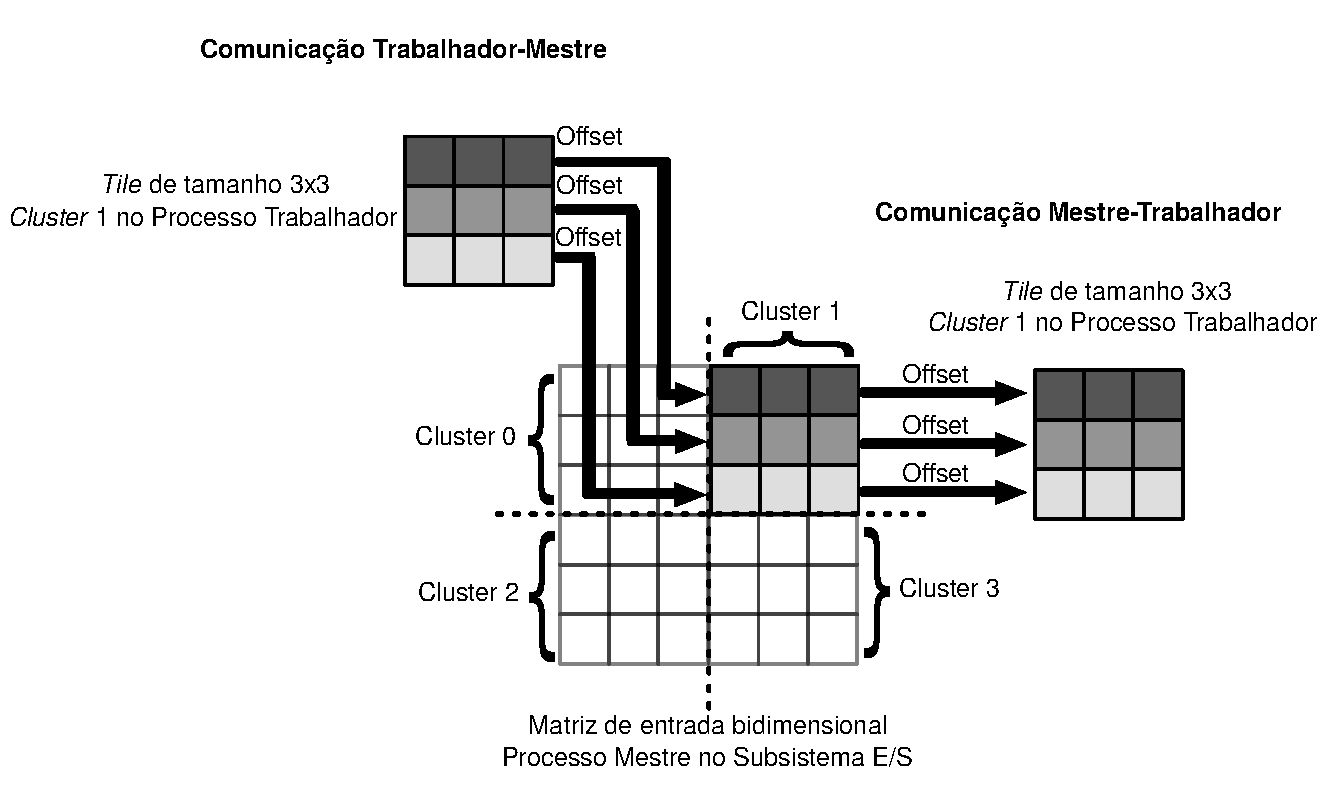
\includegraphics[width=0.7\textwidth]{figs/stridesImage.pdf}
	\caption{Exemplo do funcionamento do método \textit{strides} do \mppa.}
	\label{fig:strides}
\end{figure}

Na fase de computação, os processos trabalhadores serão responsáveis pela
execução do \textit{kernel} da computação. Essa fase pode ser dividida em
etapas: i) Cada processo trabalhador irá receber os \textit{tiles} alargados.
ii) $t^\prime$ iterações são computadas sobre o \textit{tile} alargado. iii)
\textit{offsets} são utilizados para coletar o \textit{tile} lógico e enviá-lo
ao processo mestre. Após cada \textit{tile}
atribuído ao processo trabalhador ser computado, todos os processos
trabalhadores precisam sincronizar em uma barreira. Para cumprir esse objetivo,
são utilizadas funções de baixo nível do \mppa. Esse processo é repetido até
todas as $t$ iterações serem processadas.

O código~\ref{cod:jacobiTrabalhador} mostra a definição do processo trabalhador
no \mppa. Este processo será responsável por descrever o \textit{kernel} da
computação e, também, estruturas de dados de forma similar ao processo mestre.
Devido aos valores de \textit{offsets} e variáveis importantes para a computação
do \textit{kernel} serem geradas dinâmicamente, o processo trabalhador precisa
receber do processo mestre, além do \textit{tile} alargado, variáveis
responsáveis por controlar a comunicação. Dentre elas, temos variáveis indicando
as dimensões do \textit{tile} a ser recebido, número de iterações totais e
\textit{offsets} para auxiliar a comunicação do resultado.

Por fim, para fornecer uma maior facilidade ao usuário, a técnica de
\textit{tiling} utilizada, as comunicações via \noc e adaptações foram
realizadas dentro do \textit{back-end} do \pskel.
